\documentclass[11pt]{article}
\title{\textbf{M\'etodo de Vol\'umenes Finitos}\\\textbf{Ejercicios Pr\'acticos}}
\author{Santiago Chialvo}
\date{Noviembre 20, 2015}
\usepackage{amsmath}
\usepackage{graphicx}
\usepackage[latin1]{inputenc}
\usepackage[spanish]{babel}
\usepackage[T1]{fontenc}
\usepackage{color}
\usepackage{upquote}
%\usepackage{xcolor}
\usepackage{listings}
\usepackage{caption}
\usepackage{float}

\begin{document}

\lstset{language=Matlab,%
    %basicstyle=\color{red},
    breaklines=true,%
    morekeywords={matlab2tikz},
    keywordstyle=\color{blue},%
    morekeywords=[2]{1}, keywordstyle=[2]{\color{black}},
    identifierstyle=\color{black},%
    stringstyle=\color{green},
    commentstyle=\color{red},%
    showstringspaces=false,%without this there will be a symbol in the places where there is a space
    numbers=left,%
    numberstyle={\tiny \color{black}},% size of the numbers
    numbersep=9pt, % this defines how far the numbers are from the text
    emph=[1]{for,end,break},emphstyle=[1]\color{red}, %some words to emphasise
    %emph=[2]{word1,word2}, emphstyle=[2]{style},    
}

\maketitle


\section{Problema 1: Manipuleo de Datos Geom\'etricos}

Para este ejercicio se pide que, dada una malla en formato nodos (xnod) y conectividades (icone) en 3D, se genere un c\'odigo que calcule los arreglos de OpenFOAM

\begin{itemize}
    \item (1) Faces.
    \item (2) Points.
    \item (3) Owner.
    \item (4) Neighbor.
\end{itemize}

Y las propiedades geom\'etricas 

\begin{itemize}
    \item (1) Volumen de cada celda.
    \item (2) Vector de \'Area Normal.
    \item (3) Centroide de cada Celda.
    \item (4) Centroide de cada Cara.
\end{itemize}

\bigskip A continuaci\'on se presenta el c\'odigo desarrollado y se ir\'a explicando parte por parte los pasos seguidos. El software utilizado para escribir el mismo fue Matlab.

\bigskip El array \textit{lenicone} contiene la cantidad de celdas presentes en la malla. Empezamos calculando el vol\'umen y el centroide de cada celda, dependiendo si se trata de un hexaedro o un tetraedro. Si se trata de un hexaedro, el vol\'umen se calcula dividiendo el mismo en 5 tetraedros y calculando el vol\'umen de cada uno, luego se suman.

\bigskip
\lstset{language=Matlab, breaklines=true, basicstyle=\footnotesize}
\begin{lstlisting}[frame=single]
function [faces,points,owner,neighbor,Vceldas,Cceldas,Afaces,Cfaces] = Ejercicio1_FVM(xnode,icone,hexa)

%%
%Example
%icone =  [1     2     3     4     5     6     7     8 ;5     6     7     8    9    10    11    12];
%xnode = [xnode = [0 0 0; 1 0 0; 1 1 0; 0 1 0; 0 0 0.1; 1 0 0.1; 1 1 0.1; 0 1 0.1;  0 0 0.2; 1 0 0.2; 1 1 0.2; 0 1 0.2];

points = xnode;

lenicone = length(icone(:,1)); %Cantidad de celdas

%% Calculo de volumenes y centroides de celdas

Vceldas = zeros(lenicone,1); %vector con volumenes de las celdas
Cceldas = zeros(lenicone,3); %vector con los centroides de las celdas

if (hexa)

    for i=1:lenicone
        tets = [points(icone(i,1),:) points(icone(i,2),:) points(icone(i,4),:) points(icone(i,5),:); points(icone(i,2),:) points(icone(i,4),:) points(icone(i,3),:) points(icone(i,7),:); points(icone(i,5),:) points(icone(i,2),:) points(icone(i,8),:) points(icone(i,7),:); points(icone(i,2),:) points(icone(i,5),:) points(icone(i,6),:) points(icone(i,7),:); points(icone(i,2),:) points(icone(i,5),:) points(icone(i,4),:) points(icone(i,7),:)];
        Vceldas(i) = 0;

        for j=1:5
        tet = tets(j,:);
        v1 = [tet(1) tet(2) tet(3)];
        v2 = [tet(4) tet(5) tet(6)];
        v3 = [tet(7) tet(8) tet(9)];
        v4 = [tet(10) tet(11) tet(12)];
        A = v2 - v1;
        B = v3 - v1;
        C = v4 - v1;
        mat = [A;B;C];
        Vceldas(i) = Vceldas(i) + (1/6)*abs(det(mat));
        end

        %Calcular centroide
        for j=1:8
            Cceldas(i,:) = Cceldas(i,:) + points(icone(i,j),:);
        end
        Cceldas(i,:) = Cceldas(i,:)/8;
    end

else
    
    for i=1:lenicone
        Vceldas(i) = 0;
        
        v1 = [points(icone(i,1),:) 1];
        v2 = [points(icone(i,2),:) 1];
        v3 = [points(icone(i,3),:) 1];
        v4 = [points(icone(i,4),:) 1];
        mat = [v1;v2;v3;v4];
        Vceldas(i) = (1/6)*abs(det(mat));

        %Calcular centroide
        for j=1:4
            Cceldas(i,:) = Cceldas(i,:) + points(icone(i,j),:);
        end
        Cceldas(i,:) = Cceldas(i,:)/4;
    end
    
end
\end{lstlisting}
\bigskip 

\bigskip Para cada celda, se asignan sus 4 o 6 caras correspondientes en el arreglo \textit{faces} (Siguiendo la regla de la mano derecha, todas las normales apuntando hacia afuera). Luego, en un bucle interno, se asignan todas las caras con su \textit{owner} correspondiente (Inclusive las repetidas, que ser\'an eliminadas luego).  

\bigskip
\lstset{language=Matlab, breaklines=true, basicstyle=\footnotesize}
\begin{lstlisting}[frame=single]
%% Calculo de faces y owner

if (hexa)

    faces = zeros(lenicone*6,4); % 6 caras por celda, cada una con 4 vertices
    owner = zeros(lenicone*6,1); % 6 caras, cada una con 1 propietario

    for i=1:lenicone
        faces((6*(i-1))+1,:) = [icone(i,5) icone(i,6) icone(i,7) icone(i,8)];
        faces((6*(i-1))+2,:) = [icone(i,1) icone(i,5) icone(i,8) icone(i,4)];
        faces((6*(i-1))+3,:) = [icone(i,2) icone(i,3) icone(i,7) icone(i,6)];
        faces((6*(i-1))+4,:) = [icone(i,1) icone(i,2) icone(i,6) icone(i,5)];
        faces((6*(i-1))+5,:) = [icone(i,4) icone(i,8) icone(i,7) icone(i,3)];
        faces((6*(i-1))+6,:) = [icone(i,1) icone(i,4) icone(i,3) icone(i,2)];

        for j=(6*(i-1) + 1):(6*(i-1) + 6) %Primero ponemos todas, inclusive repetidas
            owner(j) = (i);
        end
    end
    
else
    
    faces = zeros(lenicone*4,3); % 4 caras por celda, cada una con 3 vertices
    owner = zeros(lenicone*4,1); % 4 caras, cada una con 1 propietario

    for i=1:lenicone
        faces((4*(i-1))+1,:) = [icone(i,1) icone(i,3) icone(i,2)];
        faces((4*(i-1))+2,:) = [icone(i,1) icone(i,4) icone(i,3)];
        faces((4*(i-1))+3,:) = [icone(i,3) icone(i,4) icone(i,2)];
        faces((4*(i-1))+4,:) = [icone(i,1) icone(i,2) icone(i,4)];

        for j=(4*(i-1) + 1):(4*(i-1) + 4) %Primero ponemos todas, inclusive repetidas
            owner(j) = (i);
        end
    end
    
end
\end{lstlisting}
\bigskip

\bigskip Una vez inicializados estos arrays, se procede a calcular la longitud del array \textit{faces} con el fin de generar un array del mismo tama\~no, pero esta vez con cada cara con la numeraci\'on ordenada en forma ascendente. Tambi\'en creamos un array \textit{ownerdup} que ser\'a una copia exacta de \textit{owner} que ser\'a utilizado m\'as adelante para buscar caras repetidas.

\bigskip
\lstset{language=Matlab, breaklines=true, basicstyle=\footnotesize}
\begin{lstlisting}[frame=single]
lenfaces = length(faces(:,1));
if (hexa)
    facesorted = zeros(lenfaces,4);
else
    facesorted = zeros(lenfaces,3);
end
owner_dup = owner;

for i=1:lenfaces
    facesorted(i,:) = sort(faces(i,:)); %las ordeno para buscar repetidas
end
\end{lstlisting}
\bigskip

\bigskip Luego inicializar el array \textit{neighbor} en cero, inicio un bucle while en el cual, a partir de una cara del arreglo \textit{facesorted} dada, busco desde all\'i en adelante alguna otra igual. Si esto se cumple (Condici\'on if de l\'inea 9), se le asigna al array \textit{neighbor} el propietario de esa cara (Aqu\'i se utiliza el array \textit{ownerdup} dado que el \textit{owner} original cambia en cada iteraci\'on). Luego esa cara es eliminada de \textit{faces}, \textit{facesorted} y \textit{owner}. 

\bigskip
\lstset{language=Matlab, breaklines=true, basicstyle=\footnotesize}
\begin{lstlisting}[frame=single]
neighbor = zeros(1,1); %es de long variable asi que lo seteo en 1 fila
neighbor_count = 1; %para ir viendo la fila donde estoy parado

i=1;

while (i<=(lenfaces-neighbor_count+1))
    j = i+1;
    while (j<=(lenfaces-neighbor_count+1)) %busco de ahi para adelante
        if (facesorted(i,:) == facesorted(j,:)) %si encuentro una repetida
            
            neighbor(neighbor_count,1) = owner_dup(i);
            faces(j,:) = []; %lo elimino de faces
            facesorted(j,:) = []; %lo elimino de facesorted
            owner(j) = []; %lo elimino de propietarios
            neighbor_count=neighbor_count+1;
            
        end
        j=j+1;
    end
    i=i+1;
end

end
\end{lstlisting}
\bigskip

Finalmente, para el c\'alculo de el vector de \'area normal y centroide de cada cara, se recalcula la longitud del array \textit{faces} y para cada cara se utilizan f\'ormulas de \'area con vectores seg\'un se traten de hexas o tetras.

\bigskip
\lstset{language=Matlab, breaklines=true, basicstyle=\footnotesize}
\begin{lstlisting}[frame=single]
lenfaces = length(faces(:,1));

Afaces = zeros(lenfaces,3); %vector normal area de las caras
Cfaces = zeros(lenfaces,3); %centroide de las caras

if (hexa)

    for i=1:lenfaces
        v1 = points(faces(i,2),:) - points(faces(i,1),:);
        v2 = points(faces(i,4),:) - points(faces(i,1),:);
        Afaces(i,:)=cross(v1,v2);

        Cfaces(i,:) = (points(faces(i,1),:) + points(faces(i,2),:) + points(faces(i,3),:) + points(faces(i,4),:))/4;
    end

else
    
    for i=1:lenfaces
        v1 = points(faces(i,2),:) - points(faces(i,1),:);
        v2 = points(faces(i,3),:) - points(faces(i,1),:);
        Afaces(i,:)=0.5*cross(v1,v2);
        
        Cfaces(i,:) = (points(faces(i,1),:) + points(faces(i,2),:) + points(faces(i,3),:))/3;
    end
    
end
\end{lstlisting}
\bigskip

\section{Problema 2: Difusion con Fuente en 1D}

Para este problema se pide resolver la siguiente ecuaci\'on:

\begin{equation}
\int_{\Omega_j} Q^{\phi} d \Omega + \int_{\Gamma_j} \Gamma^\phi \nabla \phi \cdot d \Gamma_j = 0
\end{equation}

\bigskip En primer lugar es necesario discretizar el t\'ermino fuente y el t\'ermino difusivo. Como ya sabemos, el t\'ermino difusivo se divide en un aporte en la cara derecha y la cara izquierda, esto puede ser visto como una sumatoria para cada celda:

\begin{equation}
Q^{\phi}_c |\Omega_c| + \sum_{f = li,ld} \Gamma^\phi \nabla \phi \cdot \textbf{S}_f = 0
\end{equation}

\bigskip Finalmente, el t\'ermino $\nabla \phi$ puede ser visto como $\frac{\phi_c - \phi_w}{h}$ y el vol\'umen de la celda $|\Omega_c|$ como $S h$, reemplazando:

\begin{equation}
Q^{\phi}_c S h  + \sum_{f = li,ld} \Gamma^\phi \frac{\phi_e - \phi_c}{h} S - \Gamma^\phi \frac{\phi_c - \phi_w}{h} S = 0
\end{equation}

\bigskip

El c\'odigo que se utiliz\'o para resolver tanto \'este problema como el 3 es el mismo, s\'olo con diferentes par\'ametros. En cada sub-secci\'on se ir\'an indicando los par\'ametros elegidos y mostrando los resultados obtenidos. Al final del informe se detallar\'a el c\'odigo en cuesti\'on.

\subsection{Caso 1}

Los par\'ametros utilizados fueron:

\begin{itemize}
	\item \textit{L} = 1.
	\item \textit{tiempofinal} = 1.
    \item \textit{tipotemporal} = 3.
    \item \textit{deltaT = 1}
    \item \textit{Q} = 10.
    \item \textit{Gamma} = 1.
    \item \textit{v} = 0.
    \item \textit{rho} = 1.
    \item \textit{c (del termino reactivo)} = 0.
    \item \textit{phi0} = 0.
    \item \textit{phi1} = 1.
\end{itemize}

\bigskip Se utiliz\'o el c\'odigo con estos par\'ametros y con un h = [0.2, 0.1, 0.05, 0.025]. En la figura 1 observamos una gr\'afica del error en funci\'on del h.

\begin{figure}[tbh]
	\centering
		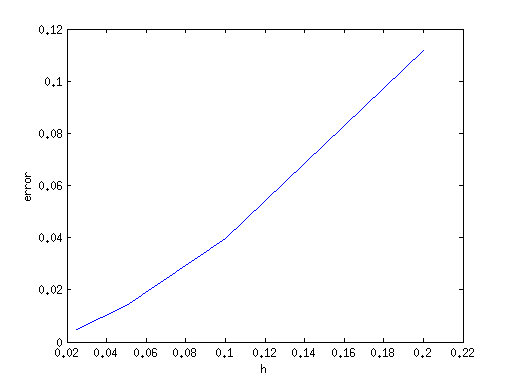
\includegraphics[width=1.0\textwidth]{imagen1.png}
	\caption{Gr\'afica del error para el caso 1}
	\label{fig:Fig1}
\end{figure}

\subsection{Caso 2}

Los par\'ametros escogidos para este caso fueron los mismos que el caso 1, s\'olo que se impuso una condici\'on Neumann en el lado izquierdo igual a 1. En este caso el error desciende con h de manera similar al caso 1. Los resultados pueden observarse en la figura 2.

\begin{figure}[tbh]
	\centering
		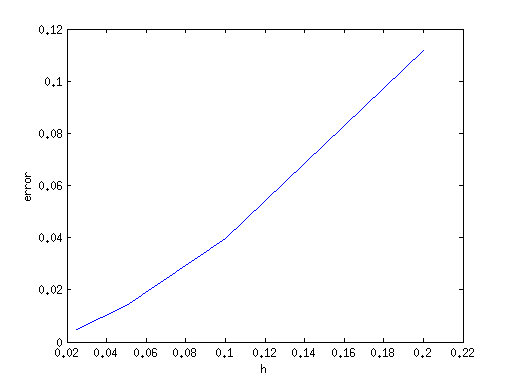
\includegraphics[width=1.0\textwidth]{imagen2.png}
	\caption{Gr\'afica del error para el caso 2}
	\label{fig:Fig1}
\end{figure}

\bigskip 
\subsection{Caso 3}

En este problema se tuvo que modificar el c\'odigo original un poco para que se genere una malla con h variable dependiendo de la siguiente funci\'on:

\begin{equation}
h = 1 - 0.75e^{\frac{(\xi - 0.5)^2}{0.01}} 
\end{equation}

Con $\xi = 0:0.01:1$

\bigskip Adem\'as se agrega una fuente variable seg\'un un intervalo. El c\'odigo utilizado para agregar esto es el siguiente:

\bigskip
\lstset{language=Matlab, breaklines=true, basicstyle=\footnotesize}
\begin{lstlisting}[frame=single]
Eta = 0:0.001:1;
lenEta = length(Eta);

h = 1 - 0.75*e.^(-((Eta-0.5).^2 ./ 0.01));
h = h/sum(h);

x(1) = 0;

for i=2:lenEta
    x(i) = x(i-1) + h(i-1);
end

cant_celdas = length(x)-1;

Q = zeros(cant_celdas,1);

for i=1:cant_celdas
    if ((x(i) >= 0.25)&&(x(i) <= 0.75))
      Q(i) = 10;  
    end
end
\end{lstlisting}
\bigskip


El resultado obtenido puedeo observarse en la figura 3.


\begin{figure}[tbh]
	\centering
		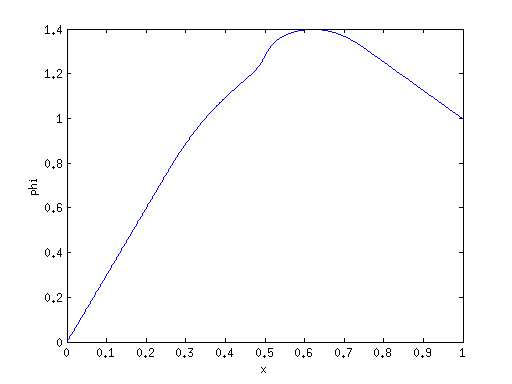
\includegraphics[width=1.0\textwidth]{imagen3.png}
	\caption{Gr\'afica de $\phi$ para el caso 3}
	\label{fig:Fig1}
\end{figure}

\bigskip 
\subsection{Caso 4}

Para este caso los par\'ametros seteados son similares al caso 1 pero la fuente Q es igual a 0.1 para todas las celdas y el valor de c en el t\'ermino reactivo es 10. El error en funci\'on del h se observa en la figura 4.

\begin{figure}[tbh]
	\centering
		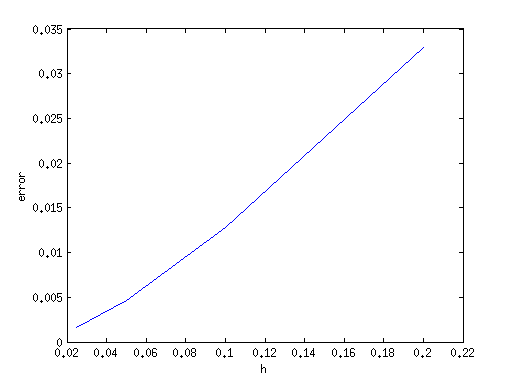
\includegraphics[width=1.0\textwidth]{imagen4.png}
	\caption{Gr\'afica del error para el caso 4}
	\label{fig:Fig1}
\end{figure}

\bigskip 
\subsection{Caso 5}

Para este caso se impuso una condici\'on mixta en el lado izquierdo con $\phi_{\inf} = 2 $ y $ h_{\inf} = 10$. El resultado obtenido puede verse en la figura 5.

\begin{figure}[tbh]
	\centering
		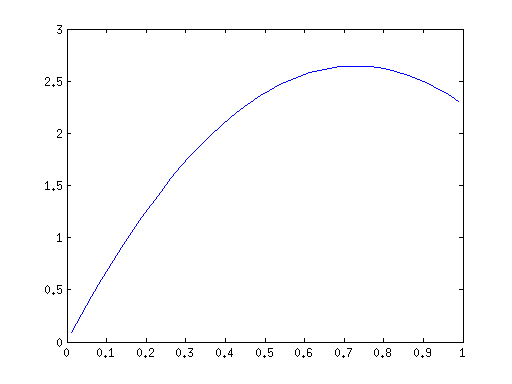
\includegraphics[width=1.0\textwidth]{imagen5.png}
	\caption{Gr\'afica de $\phi$ para el caso 5}
	\label{fig:Fig1}
\end{figure}



\section{Problema 3: Advecci\'on - Difusi\'on con fuente en 1D transiente}

Para este problema se pide resolver la siguiente ecuaci\'on:

\begin{equation}
\int_{\Omega_j} \rho \frac{d\phi}{d t} d \Omega + \int_{\Gamma_j} \rho \phi \textbf{v} \cdot d \Gamma_j  + \int_{\Omega_j} c \phi d \Omega = \int_{\Omega_j} Q^{\phi} d \Omega + \int_{\Gamma_j} \Gamma^\phi \nabla \phi \cdot d \Gamma_j
\end{equation}

\bigskip Un forma de discretizar la ecuaci\'on (5) es la siguiente:

\begin{equation}
\rho \frac{\phi^{n+1}_{c} - \phi^{n}_{c}}{\Delta t}h  + \rho v (\phi_{ld}^{n+\theta} - \phi_{li}^{n+\theta}) + c\phi_c^{n+\theta}h = Q^{\phi}_c S h  + \sum_{f = li,ld} \Gamma^\phi \frac{\phi_e - \phi_c}{h} S - \Gamma^\phi \frac{\phi_c - \phi_w}{h} S 
\end{equation}

\subsection{Caso 1}

Para este caso, se ped\'ia resolver en estado estacionario un problema con los siguientes par\'ametros:

\begin{itemize}
	\item \textit{L} = 1.
	\item \textit{tiempofinal} = 1.
    \item \textit{tipotemporal} = 3.
    \item \textit{deltaT = 1}
    \item \textit{Q} = 0.
    \item \textit{Gamma} = 1.
    \item \textit{v} = 1.
    \item \textit{rho} = 1.
    \item \textit{c (del termino reactivo)} = 0.
    \item \textit{phi0} = 0.
    \item \textit{phi1} = 1.
\end{itemize}

\bigskip La soluci\'on anal\'itica a este problema est\'a dada por la siguiente ecuaci\'on:

\begin{equation}
y(x) = \frac{(e^x-1)}{(e-1)}
\end{equation}

\bigskip El error para h = [0.2, 0.1, 0.05, 0.025] con upwind difference puede observarse en la figura 6. El orden de precisi\'on para este m\'etodo se estima en 1, es decir de primer orden, ya que el error tiende a cero como $h$. 

\bigskip El error para los mismos h pero esta vez con central difference puede observarse en la figura 7.  El orden de precisi\'on para este m\'etodo se estima en 2, es decir de segundo orden, ya que el error tiende a cero como $h^2$.

\begin{figure}[tbh]
	\centering
		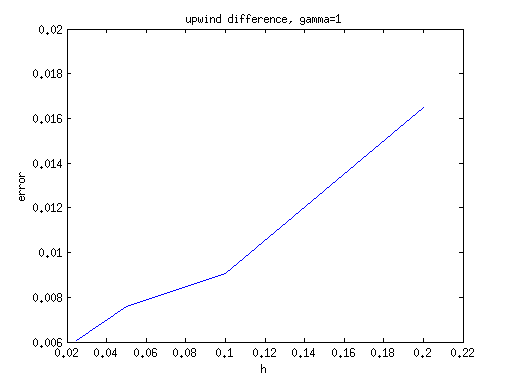
\includegraphics[width=1.0\textwidth]{imagen6.png}
	\caption{Gr\'afica del error para el caso 1 con upwind difference}
	\label{fig:Fig1}
\end{figure}

\begin{figure}[tbh]
	\centering
		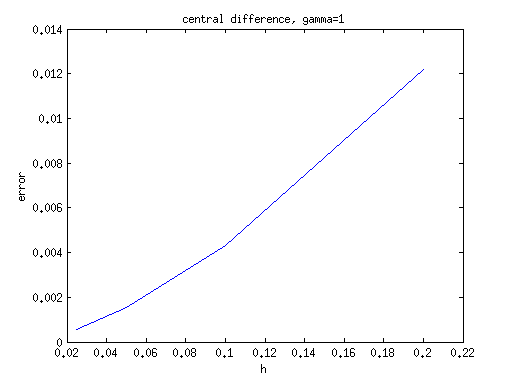
\includegraphics[width=1.0\textwidth]{imagen7.png}
	\caption{Gr\'afica del error para el caso 1 con central difference}
	\label{fig:Fig1}
\end{figure}

\subsection{Caso 2}

El mismo problema que el caso anterior, esta vez variando el t\'ermino \textit{Gamma}, en primer lugar a 0.1. En las figuras 8 y 9 observamos los resultados.

\begin{figure}[tbh]
	\centering
		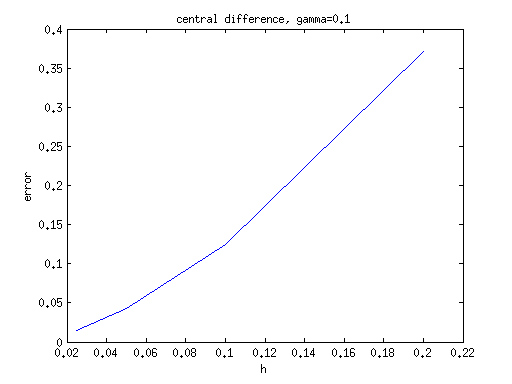
\includegraphics[width=1.0\textwidth]{imagen8.png}
	\caption{Gr\'afica del error para el caso 2, Gamma = 0.1 con upwind difference}
	\label{fig:Fig1}
\end{figure}

\begin{figure}[tbh]
	\centering
		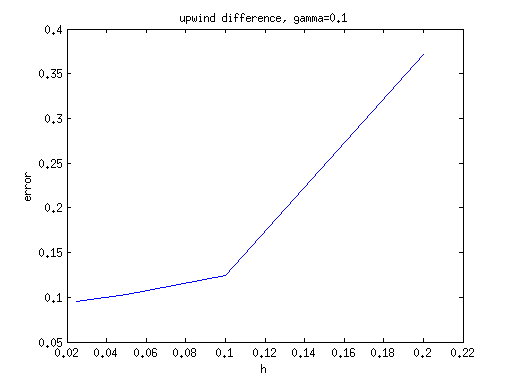
\includegraphics[width=1.0\textwidth]{imagen9.png}
	\caption{Gr\'afica del error para el caso 2, Gamma = 0.1 con central difference}
	\label{fig:Fig1}
\end{figure}

\bigskip Con un Gamma = 0.01 se tuvieron que probar varios valores m\'as de h para que se notara bien la diferencia entre \'ambos m\'etodos, desde h = 0.2 hasta h= 1.5625e-3 dividiendo h/2. Se observa como el comportamiento de central difference en la figura 10 es lineal hasta h=0.1 y luego el error desciende cuadr\'aticamente. En la figura 11 con upwind difference se observa claramente el descenso lineal del error respecto a h. 

\begin{figure}[tbh]
	\centering
		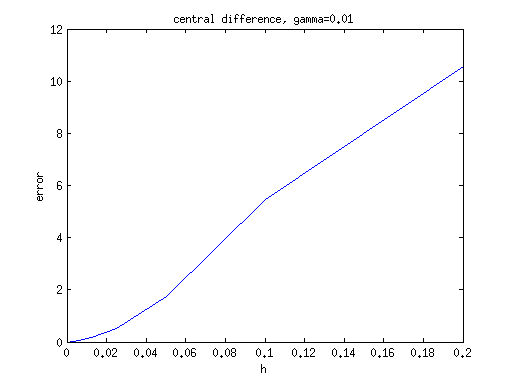
\includegraphics[width=1.0\textwidth]{imagen10.png}
	\caption{Gr\'afica del error para el caso 2, Gamma = 0.01 con central difference}
	\label{fig:Fig1}
\end{figure}

\begin{figure}[tbh]
	\centering
		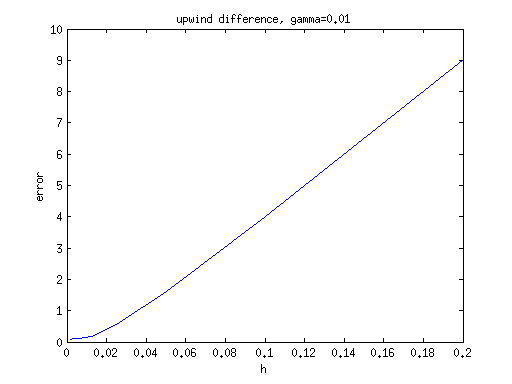
\includegraphics[width=1.0\textwidth]{imagen11.png}
	\caption{Gr\'afica del error para el caso 2, Gamma = 0.01 con upwind difference}
	\label{fig:Fig1}
\end{figure}

\subsection{Caso 3}

Para este problema, con 20 celdas no se alcanzaba a discretizar bien el gran salto que tiene la funci\'on con Gamma=0.01 entre x=[0.9,1], dando resultados totalmente imprecisos. Esto puede observarse en la figura 12. 

\begin{figure}[tbh]
	\centering
		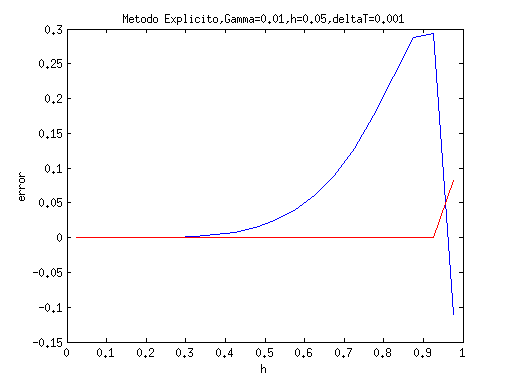
\includegraphics[width=1.0\textwidth]{imagen12.png}
	\caption{M\'etodo expl\'icito, h=0.05}
	\label{fig:Fig1}
\end{figure}

\bigskip Sin embargo, con un h = 0.005 y un deltaT = 0.001 se lograban mejores resultados. Sabemos que la elecci\'on de una deltaT adecuado es indispensable para asegurar la convergencia de \'este m\'etodo.(\textit{tipotemporal}=1) En la figura 13 se observa la gr\'afica obtenida con respecto a la soluci\'on exacta y en la figura 14 como desciende el error con el paso del tiempo. El n\'umero de Courant obtenido en este caso es de 0.2. Como el se cumple que sea menor que la unidad, el sistema expl\'icito es estable.

\begin{figure}[tbh]
	\centering
		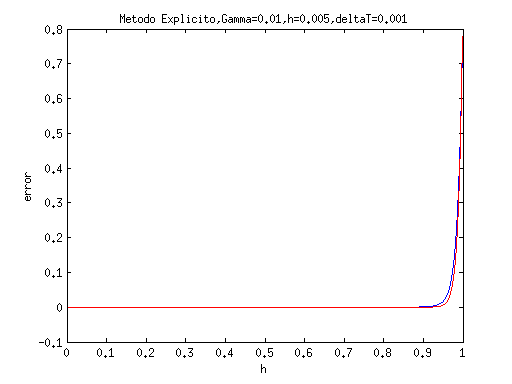
\includegraphics[width=1.0\textwidth]{imagen13.png}
	\caption{M\'etodo expl\'icito, h=0.005, deltaT = 0.001}
	\label{fig:Fig1}
\end{figure}

\begin{figure}[tbh]
	\centering
		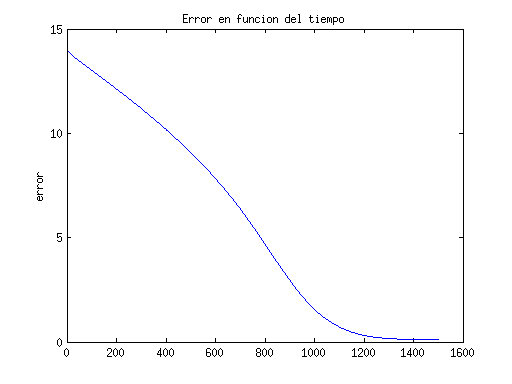
\includegraphics[width=1.0\textwidth]{imagen14.png}
	\caption{M\'etodo expl\'icito, h=0.005, deltaT = 0.001, error en funci\'on del tiempo}
	\label{fig:Fig1}
\end{figure}

\bigskip Para el caso impl\'icito, (\textit{tipotemporal}=2) no modificando ning\'un par\'ametro de los anteriores obtenemos el mismo n\'umero de Courant. Los resultados son apreciables en las figuras 15 y 16. Aumentando luego del deltaT al doble, el n\'umero de Courant aumenta consecuentemente al doble y se obtienen los resultados apreciables en las figuras 17 y 18. Los resultados son similares al caso anterior. El sistema es estable ya que no tiene limitaci\'on en el paso del tiempo en el caso lineal.

\begin{figure}[tbh]
	\centering
		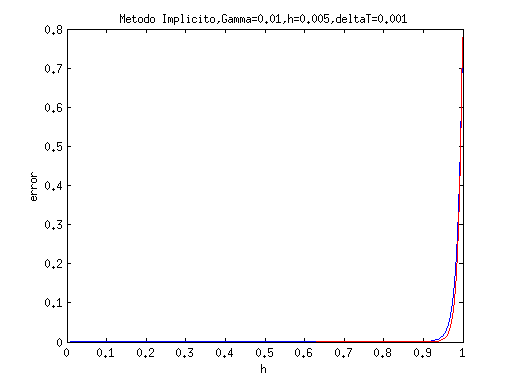
\includegraphics[width=1.0\textwidth]{imagen15.png}
	\caption{M\'etodo impl\'icito, h=0.005, deltaT = 0.001}
	\label{fig:Fig1}
\end{figure}

\begin{figure}[tbh]
	\centering
		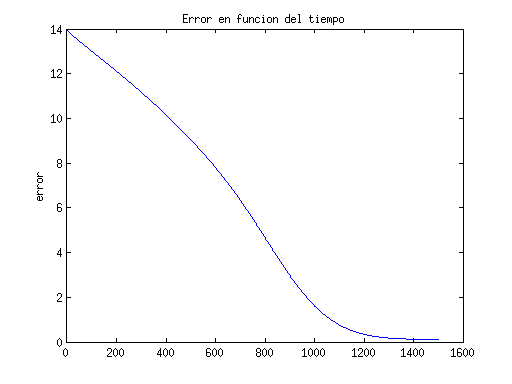
\includegraphics[width=1.0\textwidth]{imagen16.png}
	\caption{M\'etodo impl\'icito, h=0.005,, deltaT = 0.001, error en funci\'on del tiempo}
	\label{fig:Fig1}
\end{figure}

\begin{figure}[tbh]
	\centering
		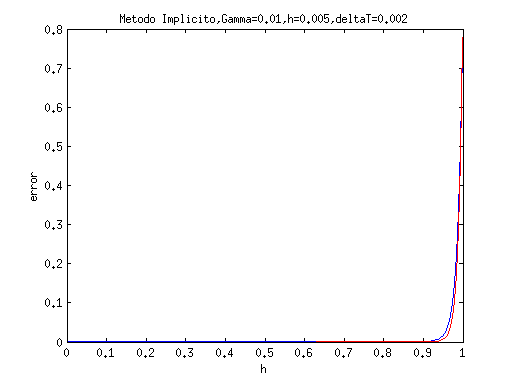
\includegraphics[width=1.0\textwidth]{imagen17.png}
	\caption{M\'etodo impl\'icito, h=0.005, deltaT = 0.002}
	\label{fig:Fig1}
\end{figure}

\begin{figure}[tbh]
	\centering
		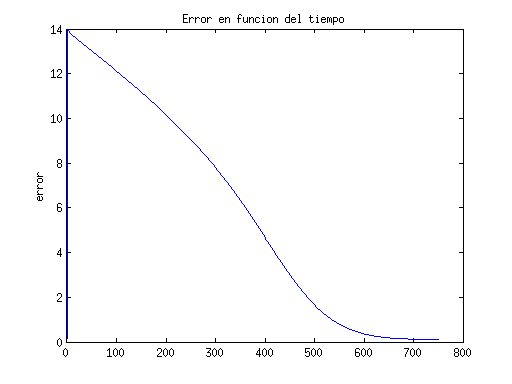
\includegraphics[width=1.0\textwidth]{imagen18.png}
	\caption{M\'etodo impl\'icito, h=0.005, deltaT = 0.002, error en funci\'on del tiempo}
	\label{fig:Fig1}
\end{figure}

\bigskip Para el tercer caso, el m\'etodo semi-expl\'icito (\textit{tipotemporal}=0) se utiliza nuevamente un deltaT = 0.001 y un h=0.005 obteniendo as\'i un Courant = 0.2, luego se usa un paso igual al doble del anterior. Los resultados son apreciables en las figuras 19,20,21 y 22.

\begin{figure}[tbh]
	\centering
		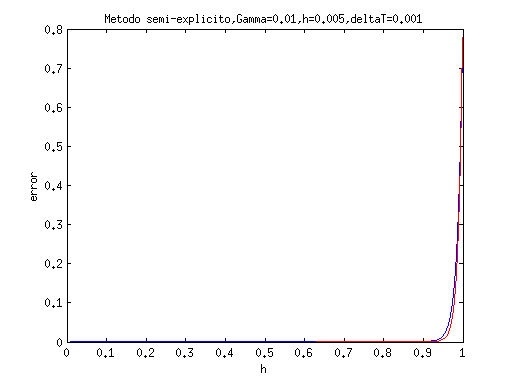
\includegraphics[width=1.0\textwidth]{imagen19.png}
	\caption{M\'etodo semi-expl\'icito, h=0.005, deltaT = 0.001}
	\label{fig:Fig1}
\end{figure}

\begin{figure}[tbh]
	\centering
		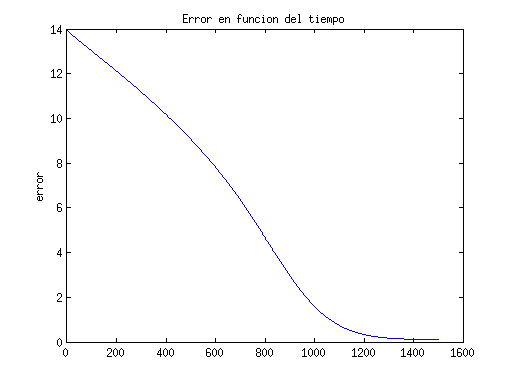
\includegraphics[width=1.0\textwidth]{imagen20.png}
	\caption{M\'etodo semi-expl\'icito, h=0.005,, deltaT = 0.001, error en funci\'on del tiempo}
	\label{fig:Fig1}
\end{figure}

\begin{figure}[tbh]
	\centering
		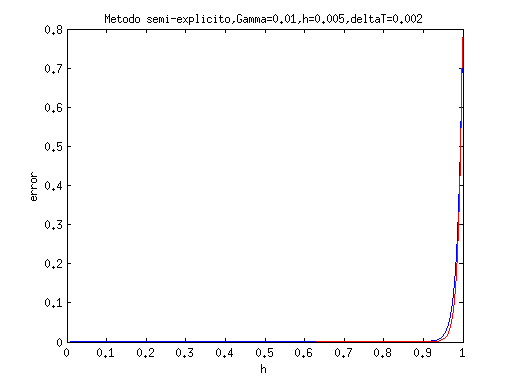
\includegraphics[width=1.0\textwidth]{imagen21.png}
	\caption{M\'etodo semi-expl\'icito, h=0.005, deltaT = 0.002}
	\label{fig:Fig1}
\end{figure}

\begin{figure}[tbh]
	\centering
		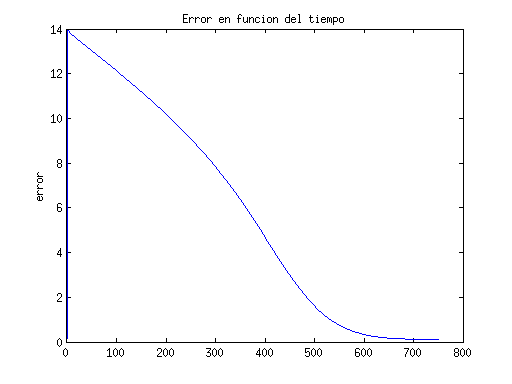
\includegraphics[width=1.0\textwidth]{imagen22.png}
	\caption{M\'etodo semi-expl\'icito, h=0.005, deltaT = 0.002, error en funci\'on del tiempo}
	\label{fig:Fig1}
\end{figure}


\section{C\'odigo utilizado}

A continuaci\'on se presenta el c\'odigo utilizado para resolver el problema 1 y 3, escrito en el software Matlab.

\bigskip
\lstset{language=Matlab, breaklines=true, basicstyle=\footnotesize}
\begin{lstlisting}[frame=single]
function [err,hvs] = TP2MC_Ej3_nuevo ()

%% Variables iniciales
h=0.005;
L = 1;
x = 0:h:L;
cant_celdas = length(x) - 1;

deltaT = 0.002;
tiempofinal = 1.5;
t = 0:deltaT:tiempofinal;
e = exp(1);

cant_tiempos = length(t);
hv = zeros(cant_celdas,1)+h;
Q = zeros(cant_celdas,1)+0;

tipotemporal = 0; %% Tipo de metodo de discretizacion temporal: 0-semi-explicito, 1-explicito, 2-implicito, 3-ninguno (estacionario)

% Termino convectivo
v = 1;
rho = 1;
upwind = true;
if (upwind)
    if (v>0)
        alfa = 1;
        beta = 0;
    else
        alfa = 0;
        beta = 1;
    end
end

%Termino reactivo
c = 0;

%Termino difusivo
Gamma = 0.01;

%Cond de borde
phi0 = 0; % izquierda
phi1 = 1; % derecha

gamabi = 1;
gamabd = 1;
hinf = 10;

cond = [0 0]; % 0-dirichlet, 1-neumann, 2-mixta

%% Inicializaciones de estructuras

K = zeros(cant_celdas,cant_celdas);
F = zeros(cant_celdas,1);
left = true;

a = zeros(cant_celdas);
a(:,1) = 1;

Courant = ((deltaT*v) / h);
disp(['Numero de Courant: ' num2str(Courant)]);
Peclet = ((h*v) / Gamma);
disp(['Numero de Peclet: ' num2str(Peclet)]);

%syms phi_left phi_cent phi_right;

%% Loop principal

for i=1:cant_celdas %cada celda
    
    for j=i:i+1 %cada cara
        
        if (j == 1) %primer cara
            %No hago nada
            left = false;
            
        else
            if (j == cant_celdas+1) %ultima cara
                %No hago nada
                
            else   
                if (left)
                    %Eq = Eq + (-1 * Gamma * (1/h) * (phi_left - phi_cent));
                    gf = hv(i)/(x(i+1) - x(i-1));
                    Gamma1 = Gamma*(1-gf) + Gamma*gf;
                    phili = rho*v;
                    
                    if (upwind)
                        K(i,j-1) = K(i,j-1) - alfa*phili;
                        K(i,j) = K(i,j) - beta*phili;
                    else
                        K(i,j) = K(i,j) - (1-gf)*rho*v;
                        K(i,j-1) = K(i,j-1) - (gf*rho*v);
                    end
                    
                    K(i,j) = K(i,j) + (Gamma1 * (1/hv(i)));
                    K(i,j-1) = K(i,j-1) - (Gamma1 * (1/hv(i)));
                    
                    
                    left = false;
                else
                    if (~left)
                        %Eq = Eq + (Gamma * (1/h) * (phi_right - phi_cent));
                        gf = hv(i)/(x(i+2) - x(i));
                        Gamma1 = Gamma*(1-gf) + Gamma*gf;
                        phild = rho*v;
                        
                        if (upwind)
                            K(i,j) = K(i,j) + beta*phild;
                            K(i,j-1) = K(i,j-1) + alfa*phild;
                        else
                            K(i,j) = K(i,j) + (gf*rho*v);
                            K(i,j-1) = K(i,j-1) + (1-gf)*rho*v;
                        end
                    
                        K(i,j) = K(i,j) - Gamma1 * (1/hv(i));
                        K(i,j-1) = K(i,j-1) + (Gamma1 * (1/hv(i)));
                        
                        left = true;
                    end
                end
            end     
        end
        
    end
    K(i,i)= K(i,i) + c*hv(i);
    F(i) = F(i) + Q(i)*hv(i);
    
end

%% Cond de contorno

h1 = hv(1)/2; % h de la primer celda
hf = hv(cant_celdas)/2; % h de la ultima celda

%Dirichlet
if (cond(1) == 0)
    %termino difusivo
    K(1,1) = K(1,1) + Gamma/h1;
    F(1) = F(1) + (Gamma*phi0)/h1;
    %termino convectivo
    F(1) = F(1) + rho*v*phi0;
end
if (cond(2) == 0)
    %termino difusivo
    K(cant_celdas,cant_celdas) = K(cant_celdas,cant_celdas) + Gamma/hf;
    F(cant_celdas) = F(cant_celdas) + (Gamma*phi1)/hf;
    %termino convectivo
    F(cant_celdas) = F(cant_celdas) - rho*v*phi1;
end

%Neumann
if (cond(1) == 1)
    %termino difusivo
    F(1) = F(1) - phi0; 
    %termino convectivo
    K(1,1) = K(1,1) - rho*v;
    F(1) = F(1) + rho*v*phi0*h1;
end
if (cond(2) == 1)
    %termino difusivo
    F(cant_celdas) = F(cant_celdas) + phi1; 
    %termino convectivo
    K(cant_celdas,cant_celdas) = K(cant_celdas,cant_celdas) + rho*v;
    F(cant_celdas) = F(cant_celdas) - rho*v*phi1*hf;
end

%Mixtas

if (cond(1) == 2)
    aux = (hinf*(gamabi/h1))/(hinf+(gamabi/h1));
    convecinf = (hinf*h1)/(gamabi+h1 * hinf);
    convecC = gamabi / (gamabi+h1 * hinf);
    %termino difusivo
    F(1) = F(1) + aux*phi0;
    K(1,1) = K(1,1) + aux;
    %termino convectivo
    K(1,1) = K(1,1) - convecC*rho*v;
    F(1) = F(1) - (convecinf*phi0)*rho*v;
end

if (cond(2) == 2)
    aux = (hinf*(gamabd/hf))/(hinf+(gamabd/hf));
    convecinf = (hinf*hf)/(gamabd+hf * hinf);
    convecC = gamabd / (gamabd+hf * hinf);
    %termino difusivo
    F(cant_celdas) = F(cant_celdas) + aux*phi1;
    K(cant_celdas,cant_celdas) = K(cant_celdas,cant_celdas) + aux;
    %termino convectivo
    K(cant_celdas,cant_celdas) = K(cant_celdas,cant_celdas) + convecC*rho*v;
    F(cant_celdas) = F(cant_celdas) + (convecinf*phi1)*rho*v;
end

%% Calculo de los centroides

for i=1:cant_celdas
    xmid(i)= x(i)+(x(i+1)-x(i))/2;
end

%% Metodo temporal
if (tipotemporal == 0) %semi explicito

terminotemporal = (rho.*hv)./deltaT;
K0(:,:) = K(:,:)./2;
Kn(:,:) = K0(:,:);

for i=1:cant_celdas 
    Kn(i,i) = Kn(i,i) + terminotemporal(i);
    K0(i,i) = K0(i,i) - terminotemporal(i);
end

for time=2:cant_tiempos
    a(:,time) = Kn(:,:)\(F(:) - (K0(:,:)*a(:,time-1)));
    
    err(time) = norm((a(:,time) - exact'));
end

else if (tipotemporal == 1) %explicito
        Faux = zeros(cant_celdas,1);
        for i = 1:cant_celdas
            Kaux(i,:) = -(deltaT/(rho*hv(i)))*K(i,:);
            Faux(i) = (deltaT/(rho*hv(i)))*F(i);
            Kaux(i,i) = Kaux(i,i)+1;
        end
        
        for time=2:cant_tiempos
            a(:,time) = Kaux*a(:,time-1) + Faux;
            
            err(time) = norm((a(:,time) - exact'));
        end
        
    else if (tipotemporal == 2) %implicito
            terminotemporal = (rho.*hv)./deltaT;
            Kaux = K;
            for i = 1:cant_celdas
                Kaux(i,i) = K(i,i) + terminotemporal(i);
            end
            Faux = F;
            
            for time=2:cant_tiempos
                Faux = F + a(:,time-1).*terminotemporal;
                
                a(:,time) = Kaux\Faux;
                
                err(time) = norm((a(:,time) - exact'));
            end
        
        else
            a(:,1) = K\F;
            err(1) = norm((a(:,1) - exact'));
        end
    end
end

%end

figure;
for i=1:cant_tiempos-1
    title(i*deltaT);
    pause(0.001);
    plot(xmid,a(:,i));
end
hold on;
plot(xmid,exact,'r');
\end{lstlisting}
\bigskip

\section{Difusi\'on con fuente en 1D estacionaria en OpenFOAM}

Para resolver este problema, primero generaremos la malla modificando el archivo \textit{blockMeshDict} del tutorial \textit{PitzDaily} de \textit{scalarTransportFoam} de la siguiente manera:

\bigskip
\lstset{language=Matlab, breaklines=true, basicstyle=\footnotesize}
\begin{lstlisting}[frame=single]
vertices
(
    (0 -0.1 -0.1)
    (1 -0.1 -0.1)
    (1 0.1 -0.1)
    (0 0.1 -0.1)
    (0 -0.1 0.1)
    (1 -0.1 0.1)
    (1 0.1 0.1)
    (0 0.1 0.1)
);

blocks
(
    hex (0 1 2 3 4 5 6 7) (50 1 1) simpleGrading (1 1 1)
);

edges
(
);

boundary
(
    side1
    {
        type patch;
        faces
        (
         	(0 4 7 3)   
        );
    }
	side2
    {
        type patch;
        faces
        (
			(1 2 6 5)
        );
    }
    empty
    {
        type empty;
        faces
        (
            (0 1 5 4)
            (5 6 7 4)
            (3 7 6 2)
            (0 3 2 1)
        );
    }
);
\end{lstlisting}
\bigskip

Para setear el Gamma en 0.1, el archivo \textit{transportPropierties} es modificado. Para un h=0.02 y deltaT=0.001 con upwind-difference se obtiene algo como se observa en las figuras 23 y 24. Para central-difference los resultados se observan en la figura 25.

\begin{figure}[tbh]
	\centering
		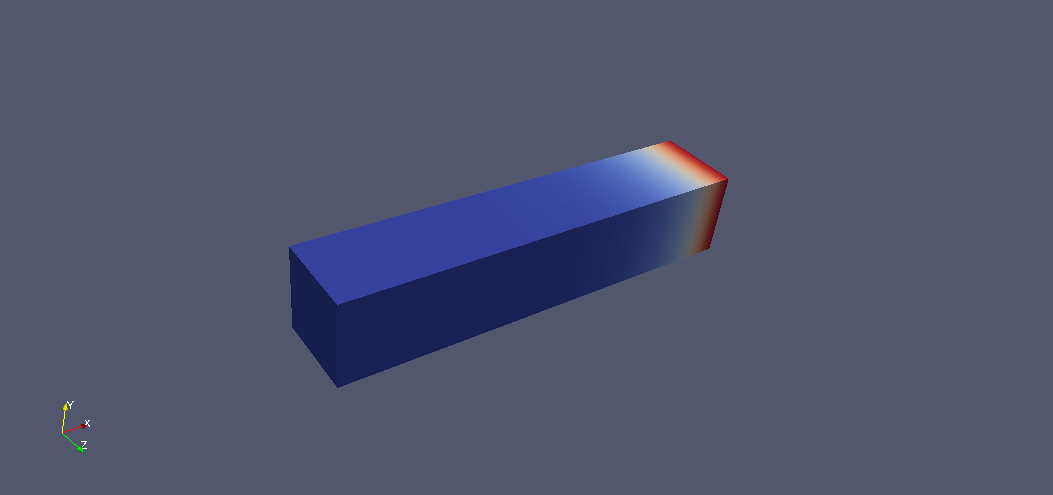
\includegraphics[width=1.0\textwidth]{imagen23.png}
	\caption{Screenshot del problema con upwind-difference y Gamma 0.1}
	\label{fig:Fig1}
\end{figure}

\begin{figure}[tbh]
	\centering
		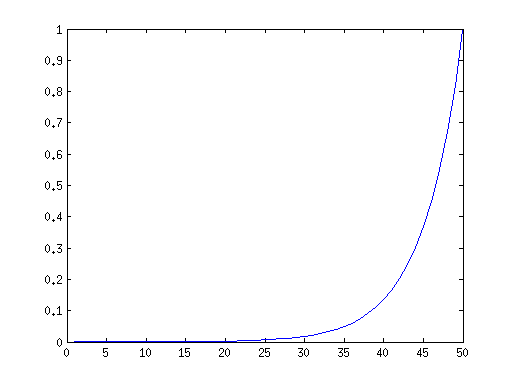
\includegraphics[width=1.0\textwidth]{imagen24.png}
	\caption{Gr\'afica de la temperatura final con upwind-difference y Gamma 0.1}
	\label{fig:Fig1}
\end{figure}

\begin{figure}[tbh]
	\centering
		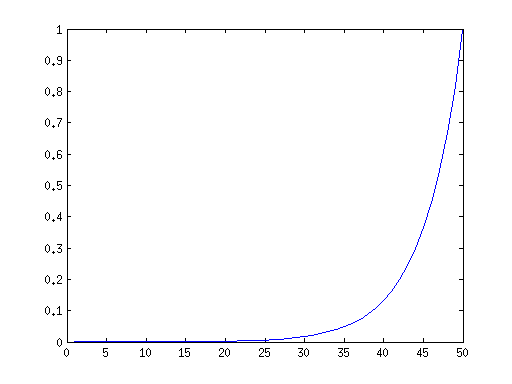
\includegraphics[width=1.0\textwidth]{imagen25.png}
	\caption{Gr\'afica de la temperatura final con central-difference y Gamma 0.1}
	\label{fig:Fig1}
\end{figure}

\bigskip De la misma manera, para un Gamma=0.01 se siguen los mismos pasos y se obtiene con upwind-difference los resultados de las figuras 26 y 27 y para CD los resultados de la imagen 28.

\begin{figure}[tbh]
	\centering
		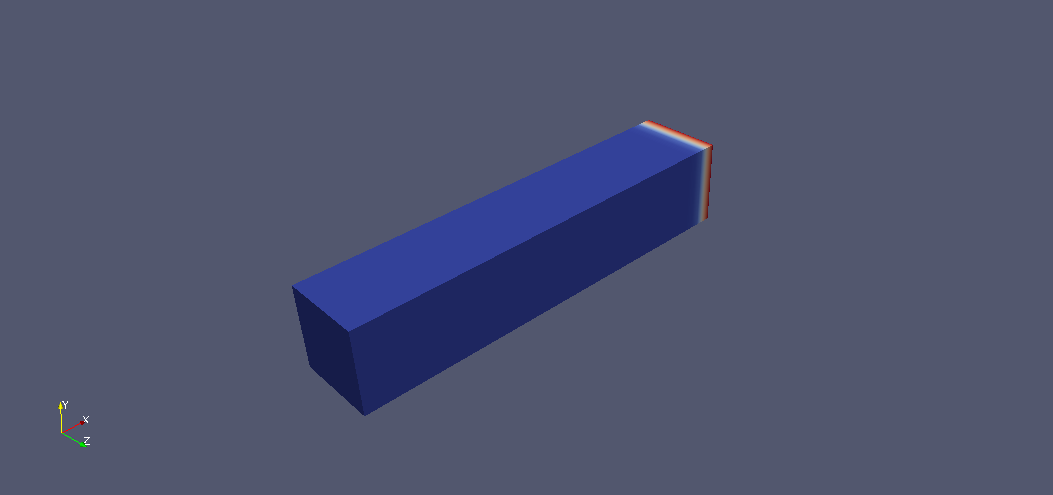
\includegraphics[width=1.0\textwidth]{imagen26.png}
	\caption{Screenshot del problema con upwind-difference y Gamma 0.01}
	\label{fig:Fig1}
\end{figure}

\begin{figure}[tbh]
	\centering
		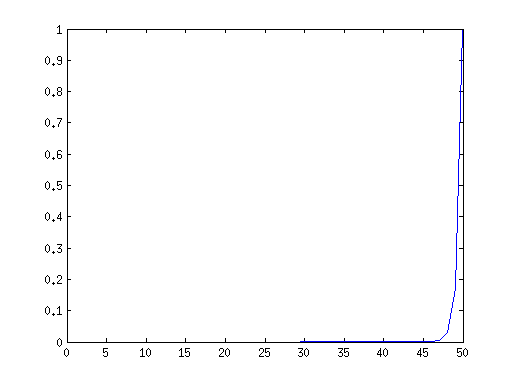
\includegraphics[width=1.0\textwidth]{imagen27.png}
	\caption{Gr\'afica de la temperatura final con upwind-difference y Gamma 0.01}
	\label{fig:Fig1}
\end{figure}

\begin{figure}[tbh]
	\centering
		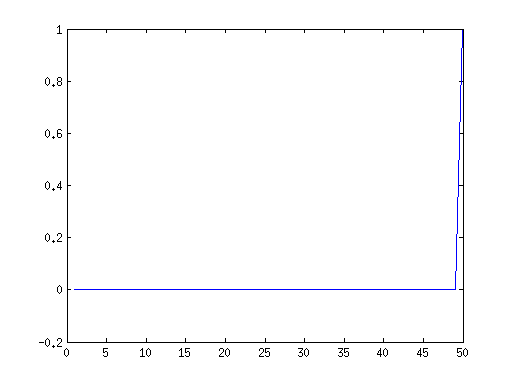
\includegraphics[width=1.0\textwidth]{imagen28.png}
	\caption{Gr\'afica de la temperatura final con central-difference y Gamma 0.01}
	\label{fig:Fig1}
\end{figure}

\bigskip Si refinamos la malla hacia el lado de x=1 usando Grading, modificamos la l\'inea correspondiente en \textit{blockMeshDict} para hacer un grading de 50 en el eje x: 

\bigskip
\lstset{language=Matlab, breaklines=true, basicstyle=\footnotesize}
\begin{lstlisting}[frame=single]
blocks
(
    hex (0 1 2 3 4 5 6 7) (50 1 1) simpleGrading (50 1 1)
);
\end{lstlisting}
\bigskip

Los resultados se observan en las figuras 29,30,31,32 y 33. En estas gr\'aficas se observa como al estar mejor discretizada la \'ultima porci\'on de la malla donde se distribuye la temperatura, el salto de temperatura que se produce en casos con el Gamma=0.01 se distribuye mejor en la gr\'afica y no se ve tan abrupto.

\begin{figure}[tbh]
	\centering
		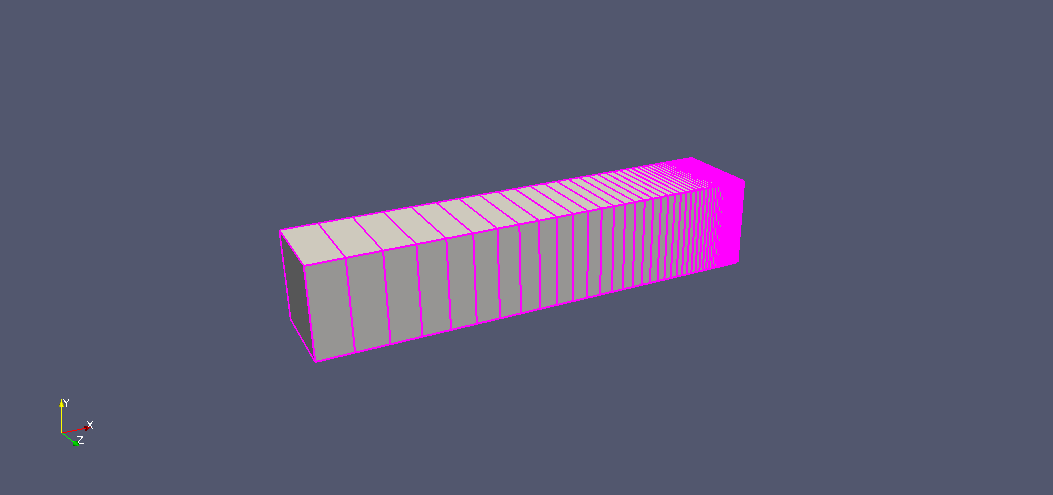
\includegraphics[width=1.0\textwidth]{imagen29.png}
	\caption{Malla refinada hacia el extremo x=L.}
	\label{fig:Fig1}
\end{figure}

\begin{figure}[tbh]
	\centering
		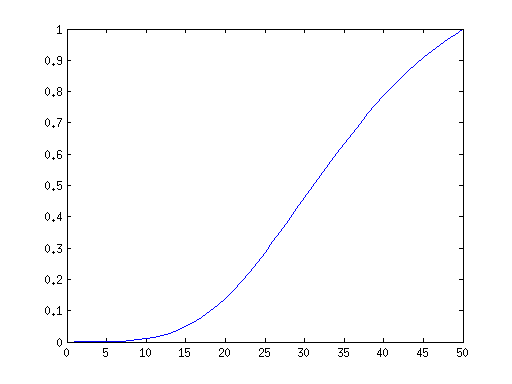
\includegraphics[width=1.0\textwidth]{imagen30.png}
	\caption{Malla refinada hacia el extremo x=L, gr\'afica de la temperatura final con upwind-difference y Gamma 0.1}
	\label{fig:Fig1}
\end{figure}

\begin{figure}[tbh]
	\centering
		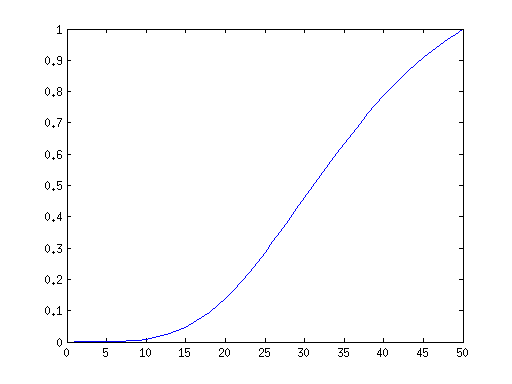
\includegraphics[width=1.0\textwidth]{imagen31.png}
	\caption{Malla refinada hacia el extremo x=L, gr\'afica de la temperatura final con central-difference y Gamma 0.1}
	\label{fig:Fig1}
\end{figure}

\begin{figure}[tbh]
	\centering
		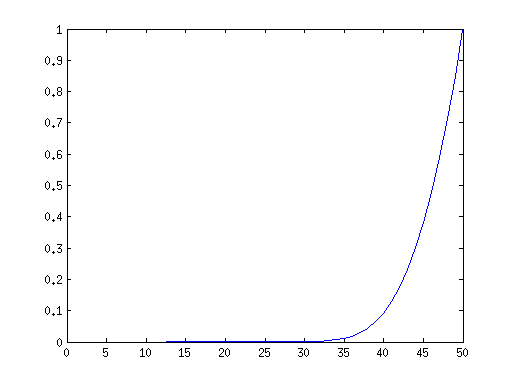
\includegraphics[width=1.0\textwidth]{imagen32.png}
	\caption{Malla refinada hacia el extremo x=L, gr\'afica de la temperatura final con upwind-difference y Gamma 0.01}
	\label{fig:Fig1}
\end{figure}

\begin{figure}[tbh]
	\centering
		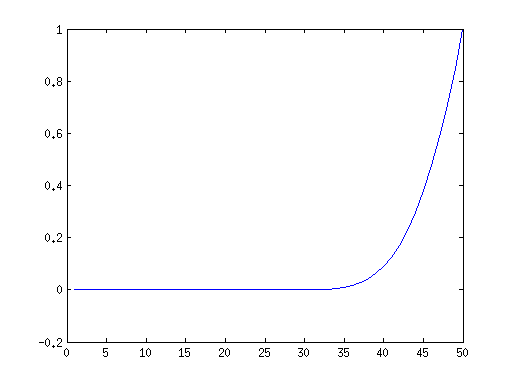
\includegraphics[width=1.0\textwidth]{imagen33.png}
	\caption{Malla refinada hacia el extremo x=L, gr\'afica de la temperatura final con central-difference y Gamma 0.01}
	\label{fig:Fig1}
\end{figure}

\section{Adveccion-Difusi\'on en 2D transiente con OpenFOAM con velocidad constante}

Para generar el dominio se modific\'o el archivo \textit{blockMeshDict} de la siguiente forma:

\bigskip
\lstset{language=Matlab, breaklines=true, basicstyle=\footnotesize}
\begin{lstlisting}[frame=single]
vertices
(
    (0 0 0)
    (1 0 0)
    (1 1 0)
    (0 1 0)
    (0 0 0.1)
    (1 0 0.1)
    (1 1 0.1)
    (0 1 0.1)
);

blocks
(
    hex (0 1 2 3 4 5 6 7) (40 40 1) simpleGrading (1 1 1)
);

edges
(
);

boundary
(
    caraarriba
    {
        type wall;
        faces
        (
            (3 7 6 2)
        );
    }
	caraizq
    {
        type wall;
        faces
        (
            (0 4 7 3)
        );
    }
    carader
    {
        type wall;
        faces
        (
            (2 6 5 1)
        );
    }
	caraabajo
    {
        type wall;
        faces
        (
            (1 5 4 0)
        );
    }
    frontAndBack
    {
        type empty;
        faces
        (
            (0 3 2 1)
            (4 5 6 7)
        );
    }
);
\end{lstlisting}
\bigskip

Luego de setear las temperaturas y la velocidades correspondientes en la carpeta 0 y $\Gamma$ en la carpeta \textit{Constant} los resultados obtenidos fueron los siguientes (Figuras 34,35,36 y 37). Al ser Gamma tan peque\~no, la temperatura no llega a distribuirse de manera completa en todo el dominio. Si aumentamos Gamma a 1, observamos un transporte de temperatura mas distribuido como se observa en la figura 38.

\begin{figure}[tbh]
	\centering
		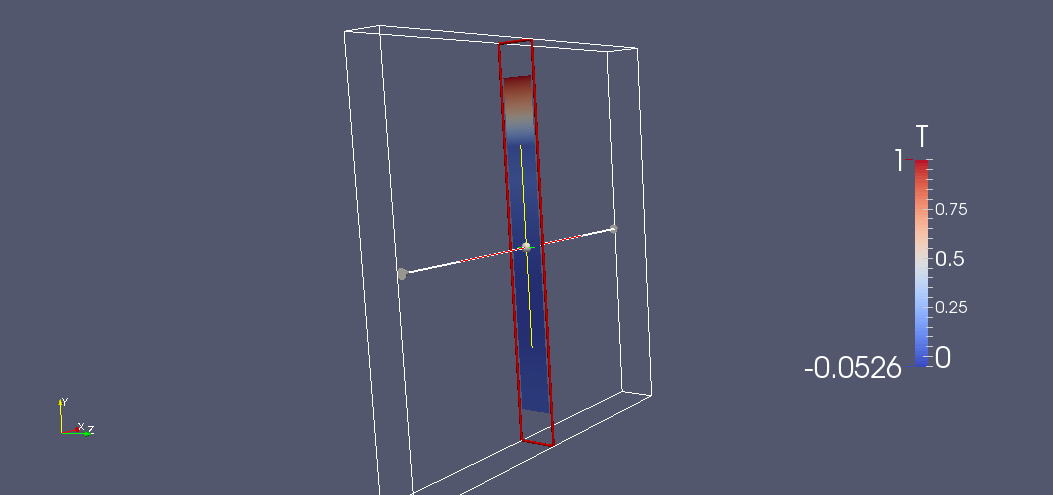
\includegraphics[width=1.0\textwidth]{imagen34.png}
	\caption{Corte de la soluci\'on en x = 1/2, N=40}
	\label{fig:Fig1}
\end{figure}

\begin{figure}[tbh]
	\centering
		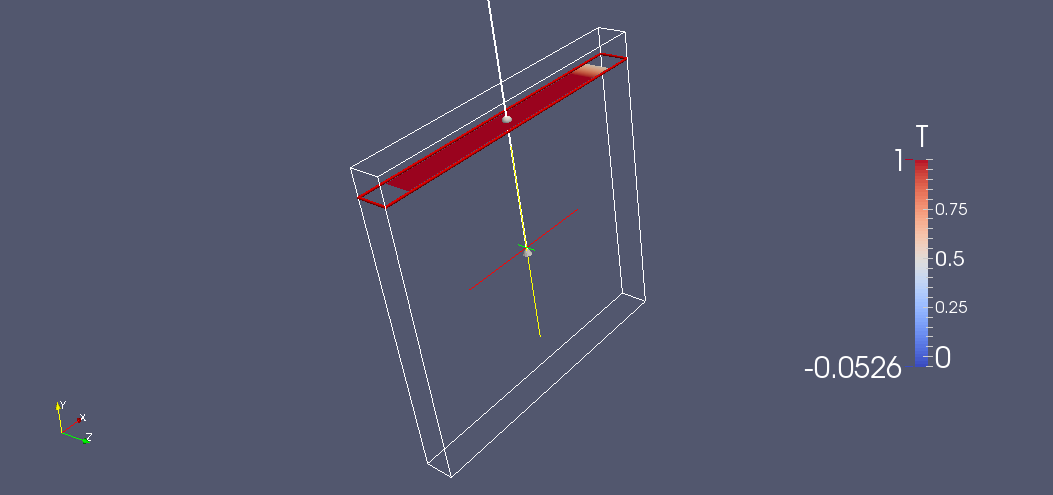
\includegraphics[width=1.0\textwidth]{imagen35.png}
	\caption{Corte de la soluci\'on en y = 1, N=40}
	\label{fig:Fig1}
\end{figure}

\begin{figure}[tbh]
	\centering
		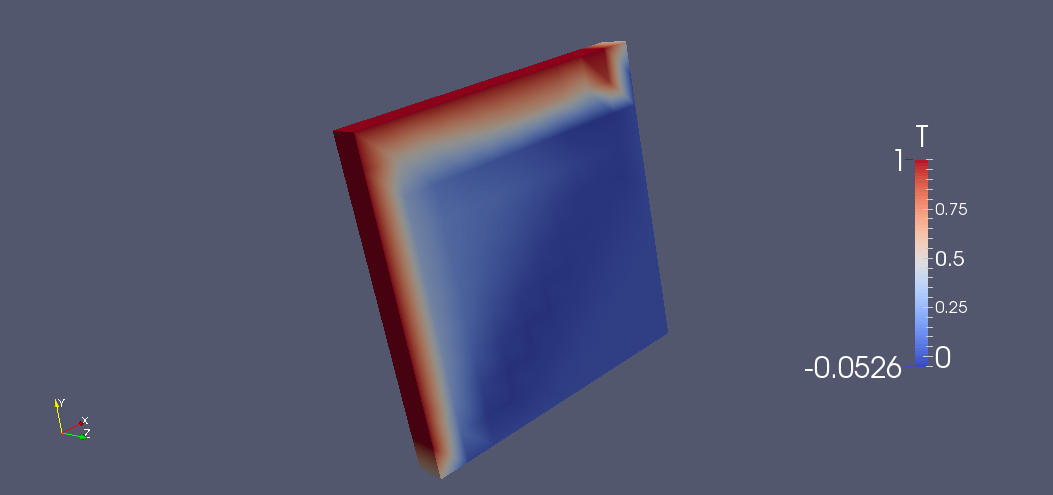
\includegraphics[width=1.0\textwidth]{imagen36.png}
	\caption{Funci\'on $\phi$ en todo el dominio, N=40}
	\label{fig:Fig1}
\end{figure}

\begin{figure}[tbh]
	\centering
		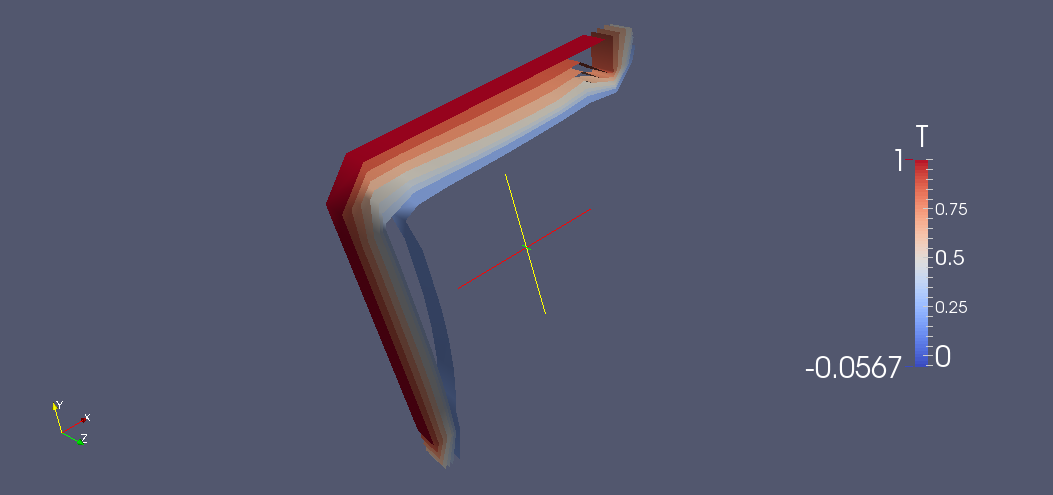
\includegraphics[width=1.0\textwidth]{imagen37.png}
	\caption{Distintas isotermas de la funci\'on $\phi$, N=40}
	\label{fig:Fig1}
\end{figure}

\begin{figure}[tbh]
	\centering
		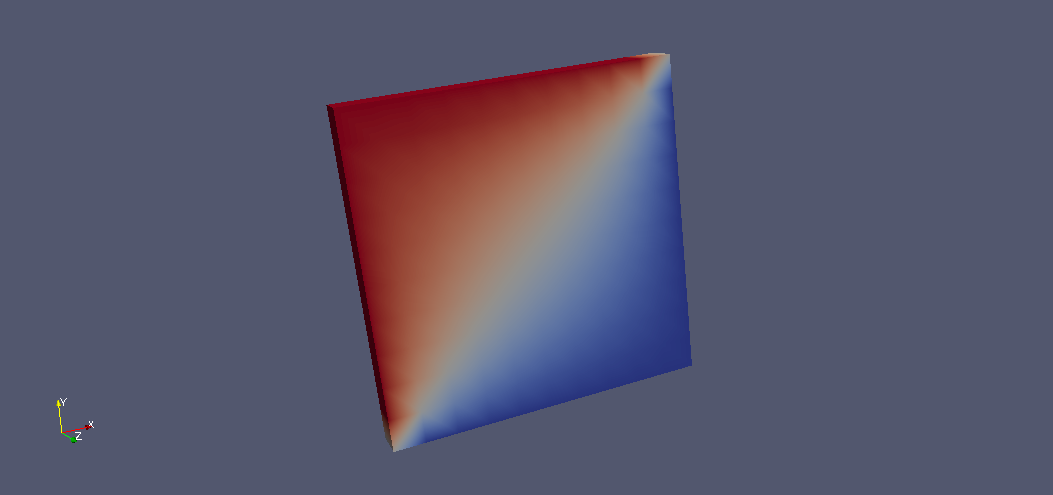
\includegraphics[width=1.0\textwidth]{imagen38.png}
	\caption{Funci\'on $\phi$ en todo el dominio con Gamma=1, N=40}
	\label{fig:Fig1}
\end{figure}

\section{Adveccion-Difusi\'on en 2D transiente con OpenFOAM con velocidad variable en el espacio}

En primer lugar, para lograr el n\'umero de Raynolds pedido la viscosidad cinem\'atica debe ser seteada en 0.0025, en el archivo \textit{transportProperties}. Una vez convergido el campo de velocidades, se obtiene lo que se observa en la figura 39.

\begin{figure}[tbh]
	\centering
		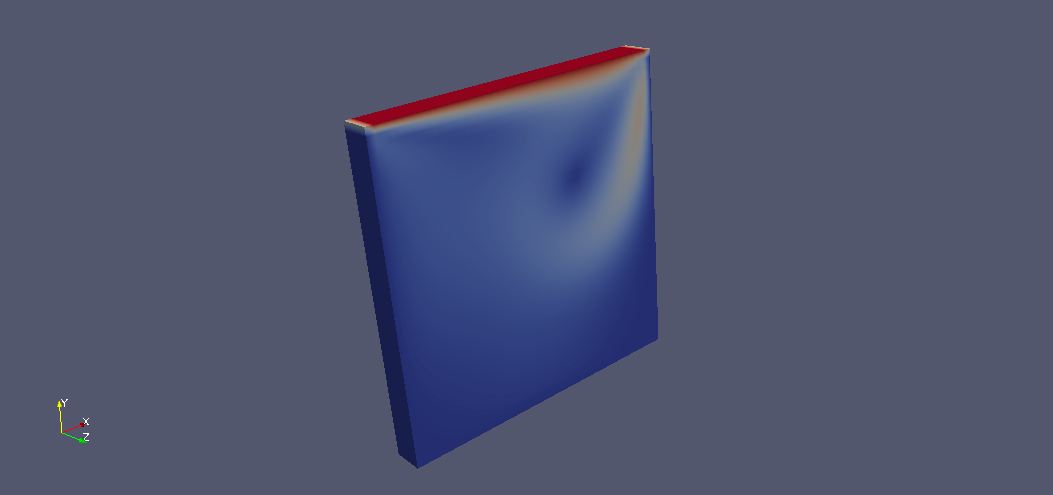
\includegraphics[width=1.0\textwidth]{imagen39.png}
	\caption{Campo de velocidades obtenido con la soluci\'on convergida}
	\label{fig:Fig1}
\end{figure}

\bigskip Con este campo de velocidades, debemos armar un caso que resuelva el transporte de la temperatura usando el campo de velocidades hallado. Para ello, en nuestro nuevo caso debemos modificar el archivo U de la carpeta 0, y setear nuestro campo de velocidades encontrado como elcampo interno de velocidades del nuevo caso. Para setear las temperaturas se modific\'o el archivo T en la carpeta 0 de la siguiente forma:

\bigskip
\lstset{language=Matlab, breaklines=true, basicstyle=\footnotesize}
\begin{lstlisting}[frame=single]
internalField   uniform 0;

boundaryField
{
	carasuperior
    {
        type            fixedGradient;
		gradient		uniform 100;
    }
	lateralizquierda
    {
        type            fixedValue;
		value			uniform 100;
    }
    lateralderecha
    {
        type            fixedValue;
		value			uniform 200;
    }
	carainferior
    {
        type            zeroGradient;
    }
    frontAndBack
    {
        type empty;
    }
}
\end{lstlisting}
\bigskip

El campo de temperatura obtenido puede observarse en la figura 40. Distintas isotermas del mismo pueden verse en la figura 41. Aqu\'i observamos como las isotermas son rectas en la pared inferior adiab\'atica y la temperatura superior se halla en el extremo superior derecho, dado que el campo de velocidades la transporta hacia ese extremo.

\begin{figure}[tbh]
	\centering
		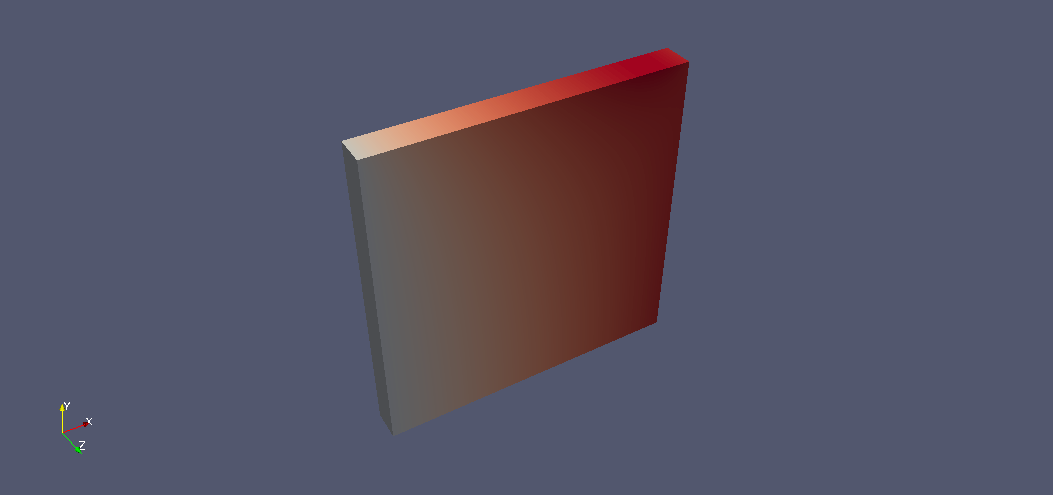
\includegraphics[width=1.0\textwidth]{imagen40.png}
	\caption{Screenshot del campo de temperaturas distribuido obtenido}
	\label{fig:Fig1}
\end{figure}

\begin{figure}[tbh]
	\centering
		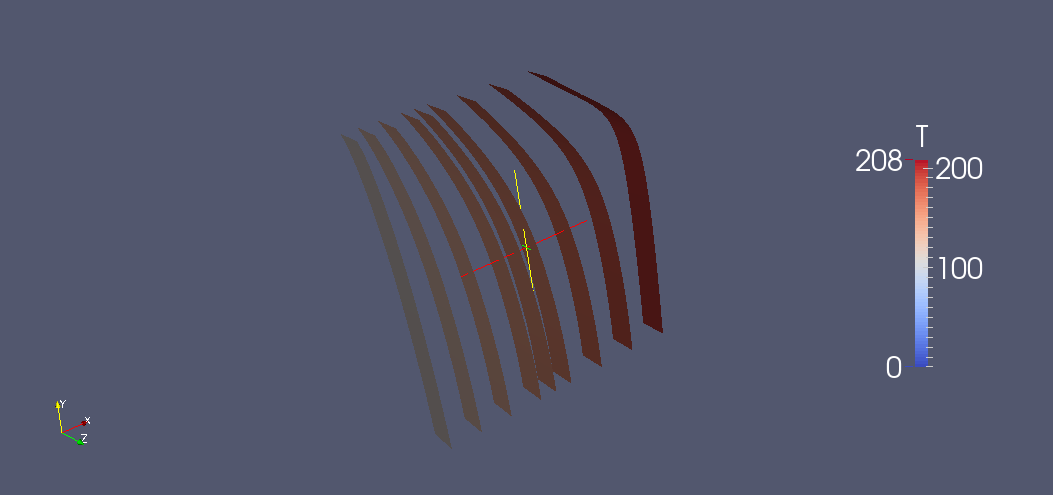
\includegraphics[width=1.0\textwidth]{imagen41.png}
	\caption{Diferentes isotermas para el campo de temperaturas obtenido}
	\label{fig:Fig1}
\end{figure}


\end{document}
